\documentclass{beamer}

\usepackage{graphicx}

\usepackage{fancyvrb} 
\newcommand\userinput[1]{\textbf{#1}}
\usepackage{tgcursor}

\usepackage{tikz}
\usetikzlibrary{arrows,shapes}

\usepackage{minted}
\usepackage{xcolor} 
\definecolor{LightGray}{gray}{0.975}

\title{Database System Concepts, $7^{th}$ Ed. \\Chapter 1: Introduction}
\author{Silbershcatz, Korth and Sudarshan}
\date{\today}

%\usetheme{Warsaw}
\usefonttheme{serif} 

\title[Chapter 1]{Database System Concepts, $7^{th}$ Edition \\ Chapter 1: Introduction}
\author{Silberschatz, Korth and Sudarshan}
\date{\today}

\setbeamertemplate{navigation symbols}{}%remove navigation symbols

\defbeamertemplate*{footline}{shadow theme}
{%
  \leavevmode%
  \hbox{\begin{beamercolorbox}[wd=.5\paperwidth,ht=2.5ex,dp=1.125ex,leftskip=.3cm plus1fil,rightskip=.3cm]{author in head/foot}%
    \usebeamerfont{author in head/foot} Database System Concepts \hfill \insertshorttitle
  \end{beamercolorbox}%
  \begin{beamercolorbox}[wd=.5\paperwidth,ht=2.5ex,dp=1.125ex,leftskip=.3cm,rightskip=.3cm plus1fil]{title in head/foot}%
    \usebeamerfont{title in head/foot} \hfill \insertframenumber\,/\,\inserttotalframenumber%
  \end{beamercolorbox}}%
  \vskip0pt%
}

\AtBeginSection[]
  {
     \begin{frame}<beamer>
     \frametitle{Plan}
     \tableofcontents[currentsection]
     \end{frame}
  }


\begin{document}

\frame{\titlepage}

\begin{frame}{Database System Concepts}
    \centering
    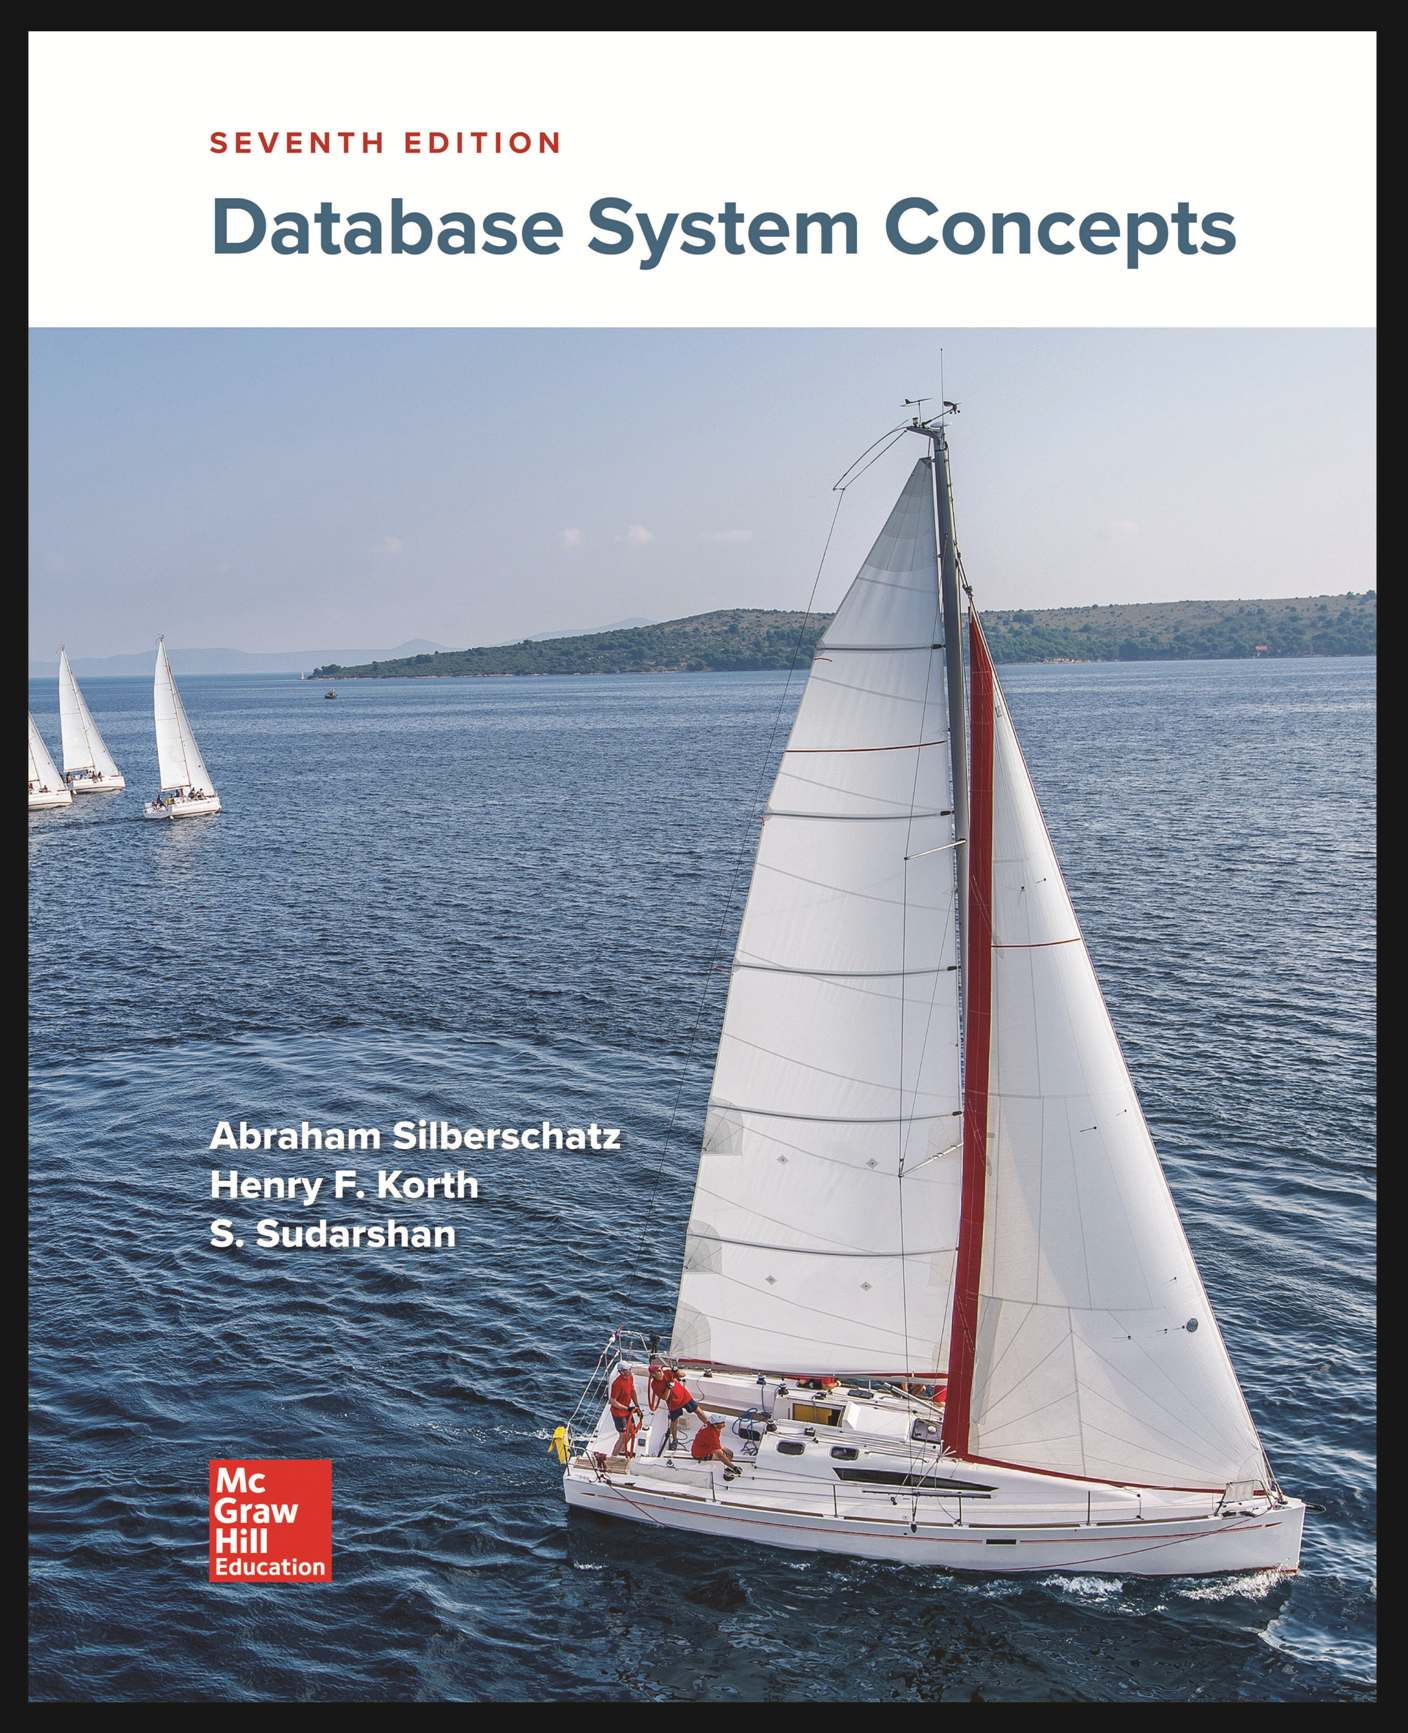
\includegraphics[width=0.5\textwidth]{figures/book_cover.jpg} \\
    \vspace{5mm}
    {
        \tiny
        Content has been extracted from \textit{Database System Concepts}, Seventh Edition, by Silberschatz, Korth and Sudarshan. Mc Graw Hill Education. 2019.\\
        Visit \url{https://db-book.com/}.\\
    }
\end{frame}

\section{Database Systems Applications}

\begin{frame}{Database Systems Applications}
    \begin{itemize}
        \item DBMS contains information about a particular enterprise:
        \begin{itemize}
            \item Collection of interrelated data.
            \item Set of programs to access the data.
            \item An environment that is both \textit{convenient} and \textit{efficient} to use.
        \end{itemize}
        \item Database systems manage collections of data that are:
        \begin{itemize}
            \item Highly valuable
            \item Relatively large
            \item Accessed by multiple users and applications, often at the same time
        \end{itemize}
        \item A modern database system is a complex software system tasked with managing a large, complex collection of data.
        \item Databases touch all aspects of our lives.
    \end{itemize}
\end{frame}

\begin{frame}{Database Applications Examples}
\begin{itemize}
    \item Enterprise Information:
    \begin{itemize}
        \item Sales: customers, products, purchases.
        \item Accounting: payments, receipts, assets.
        \item Human Resources: Information about employees, salaries, payroll taxes.
        \item Manufacturing: management of production, inventory, orders, supply chain.
    \end{itemize}
    \item Banking and Finance:
    \begin{itemize}
        \item Customer information, accounts, loans, and banking transactions.
        \item Credit card transactions.
        \item Finance: sales and purchases of financial instruments (e.g. stocks and bonds, real-time market data, ...)
    \end{itemize}
    \item Universities:
    \begin{itemize}
        \item Registration, grades
    \end{itemize}
\end{itemize}
\end{frame}

\begin{frame}{Database Applications Examples (Cont.)}
    \begin{itemize}
        \item Airlines: reservations, schedules
        \item Telecommunication: records of calls, texts, data usage, generating bills.
        \item Web-based services:
        \begin{itemize}
            \item Online retailers: order tracking, customized recommendations.
            \item Online advertisements.
        \end{itemize}
        \item Document databases.
        \item Navigation systems: locations of places of interest, routes, transport systems, etc.
    \end{itemize}
\end{frame}

\section{Purpose of Database Systems}

\begin{frame}{Purpose of Database Systems}
    In the early days, database applications were built directly on top of file systems, which leads to:
    \begin{itemize}
        \item Data redundancy and inconsistency: data is stored  in multiple file formats resulting in duplication of information in different files.
        \item Difficulty in accessing data:
        \begin{itemize}
            \item New program needed for every new task.
        \end{itemize}
        \item Data isolation:
        \begin{itemize}
            \item Multiple files and formats
        \end{itemize}
        \item Integrity problems:
        \begin{itemize}
            \item Integrity constraints  (e.g., account balance $>$ 0) become ``buried'' in program code rather than being stated explicitly.
            \item Hard to add new constraints or change existing ones.
        \end{itemize}
    \end{itemize}
\end{frame}

\begin{frame}{Purpose of Database Systems (Cont.)}
    \begin{itemize}
        \item Atomicity of updates:
        \begin{itemize}
            \item Failures may leave database in an inconsistent state with partial updates carried out.
            \item Example: Transfer of funds from one account to another should either complete or not happen at all.
        \end{itemize}
        \item Concurrent access by multiple users:
        \begin{itemize}
            \item Concurrent access needed for performance.
            \item Uncontrolled concurrent accesses can lead to inconsistencies.
            \item Ex: Two people reading a balance (say 100) and updating it by withdrawing money (say 50 each) at the same time.
        \end{itemize}
        \item Security problems:
        \begin{itemize}
            \item Hard to provide user access to some, but not all, data.
        \end{itemize}
    \end{itemize}
    \vspace{5mm}
    \centering
    \textbf{Database systems offer solutions to all the above problems.}
\end{frame}

\begin{frame}{University Database Example}
    \begin{itemize}
        \item We will be using a university database to illustrate all the concepts.
        \item Data consists of information about:
        \begin{itemize}
            \item Students
            \item Instructors
            \item Classes
        \end{itemize}
        \item Application program examples:
        \begin{itemize}
            \item Add new students, instructors, and courses.
            \item Register students for courses, and generate class rosters.
            \item Assign grades to students, compute grade point averages (GPA) and generate transcripts.
        \end{itemize}
    \end{itemize}
\end{frame}

\section{View of Data}

\begin{frame}{View of Data}
    \begin{itemize}
        \item A database system is a collection of interrelated data and a set of programs that allow users to access and modify these data. 
        \item A major purpose of a database system is to provide users with an abstract view of the data.
        \begin{itemize}
            \item Data models:
            \begin{itemize}
                \item A collection of conceptual tools for describing data, data relationships, data semantics, and consistency constraints.
            \end{itemize}
            \item Data abstraction:
            \begin{itemize}
                \item Hide the complexity  of data structures to represent data in the database from users through several levels of data abstraction.
            \end{itemize}
        \end{itemize}
    \end{itemize}
\end{frame}

\section{Data Models}
\begin{frame}{Data Models}
    \begin{itemize}
        \item A collection of tools for describing:
        \begin{itemize}
            \item Data.
            \item Data relationships.
            \item Data semantics.
            \item Data constraints.
        \end{itemize}
        \item Relational model.
        \item Entity-Relationship data model (mainly for database design) .
        \item Object-based data models (Object-oriented and Object-relational)
        \item Semi-structured data model  (XML).
        \item Other older models:
        \begin{itemize}
            \item Network model.
            \item Hierarchical model
        \end{itemize}
    \end{itemize}
\end{frame}

\section{Relational Data Model}
\begin{frame}{Relational Data Model}
    \begin{itemize}
        \item All the data is stored in various tables.
        \item Example of tabular data in the relational model:
    \end{itemize}
    \begin{minipage}{.5\textwidth}
        \centering
        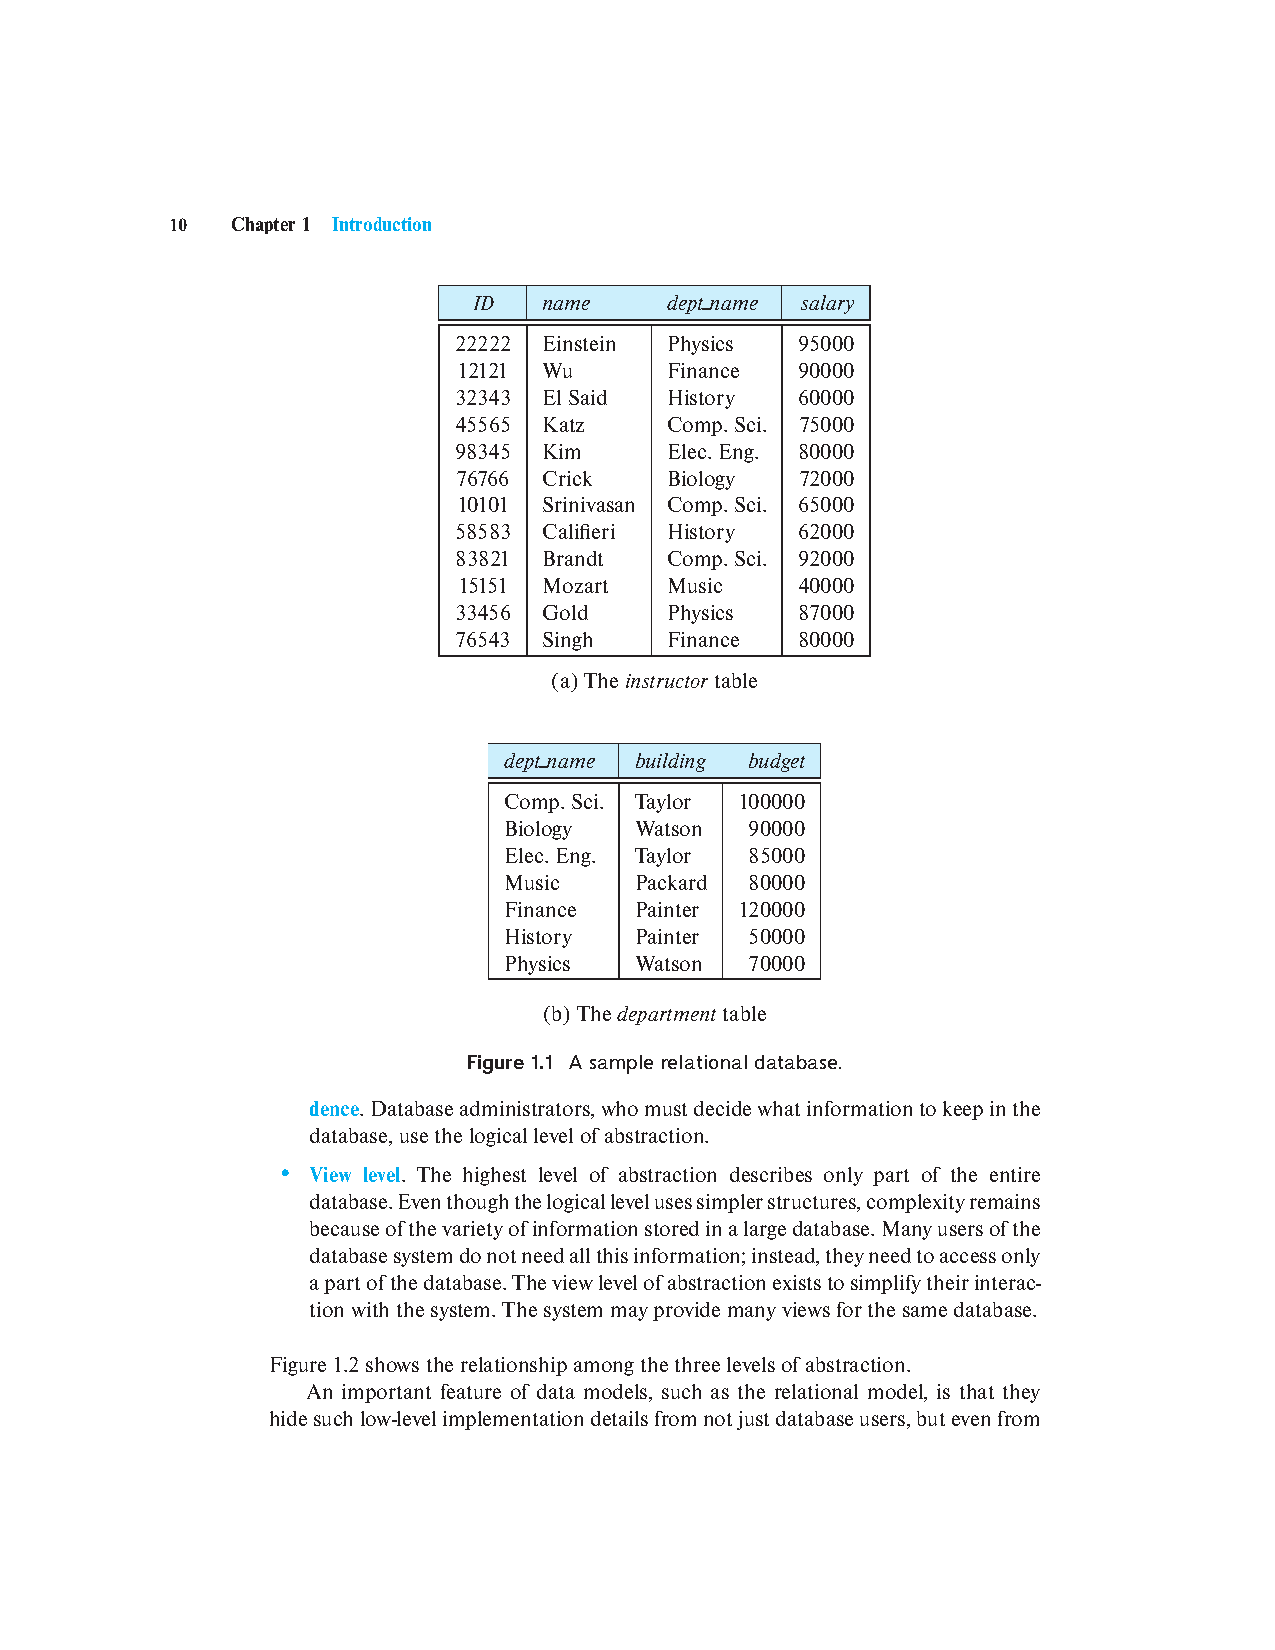
\includegraphics[width=\textwidth, trim={7cm 16cm 6.5cm 4cm}, clip]{figures/db}
    \end{minipage}%
    \begin{minipage}{0.5\textwidth}
        \centering
        \includegraphics[width=0.5\linewidth]{figures/codd}\\
        \textbf{Ted Codd}\\
        Turing Award 1981
    \end{minipage}
    \begin{tikzpicture}[remember picture,overlay]   %% use here too
        \node[] at (3.5, 5.33) {\tiny Column};
        \draw[red,thick,->] (3.5,5.225) -- (3.5,4.75);
        \node[] at (5.75, 0.76) {\tiny Row};
        \draw[blue,thick,->] (5.5, 0.76) -- (5.05, 0.76);
    \end{tikzpicture}
\end{frame}

\begin{frame}{A Sample Relational Database}
    \centering 
    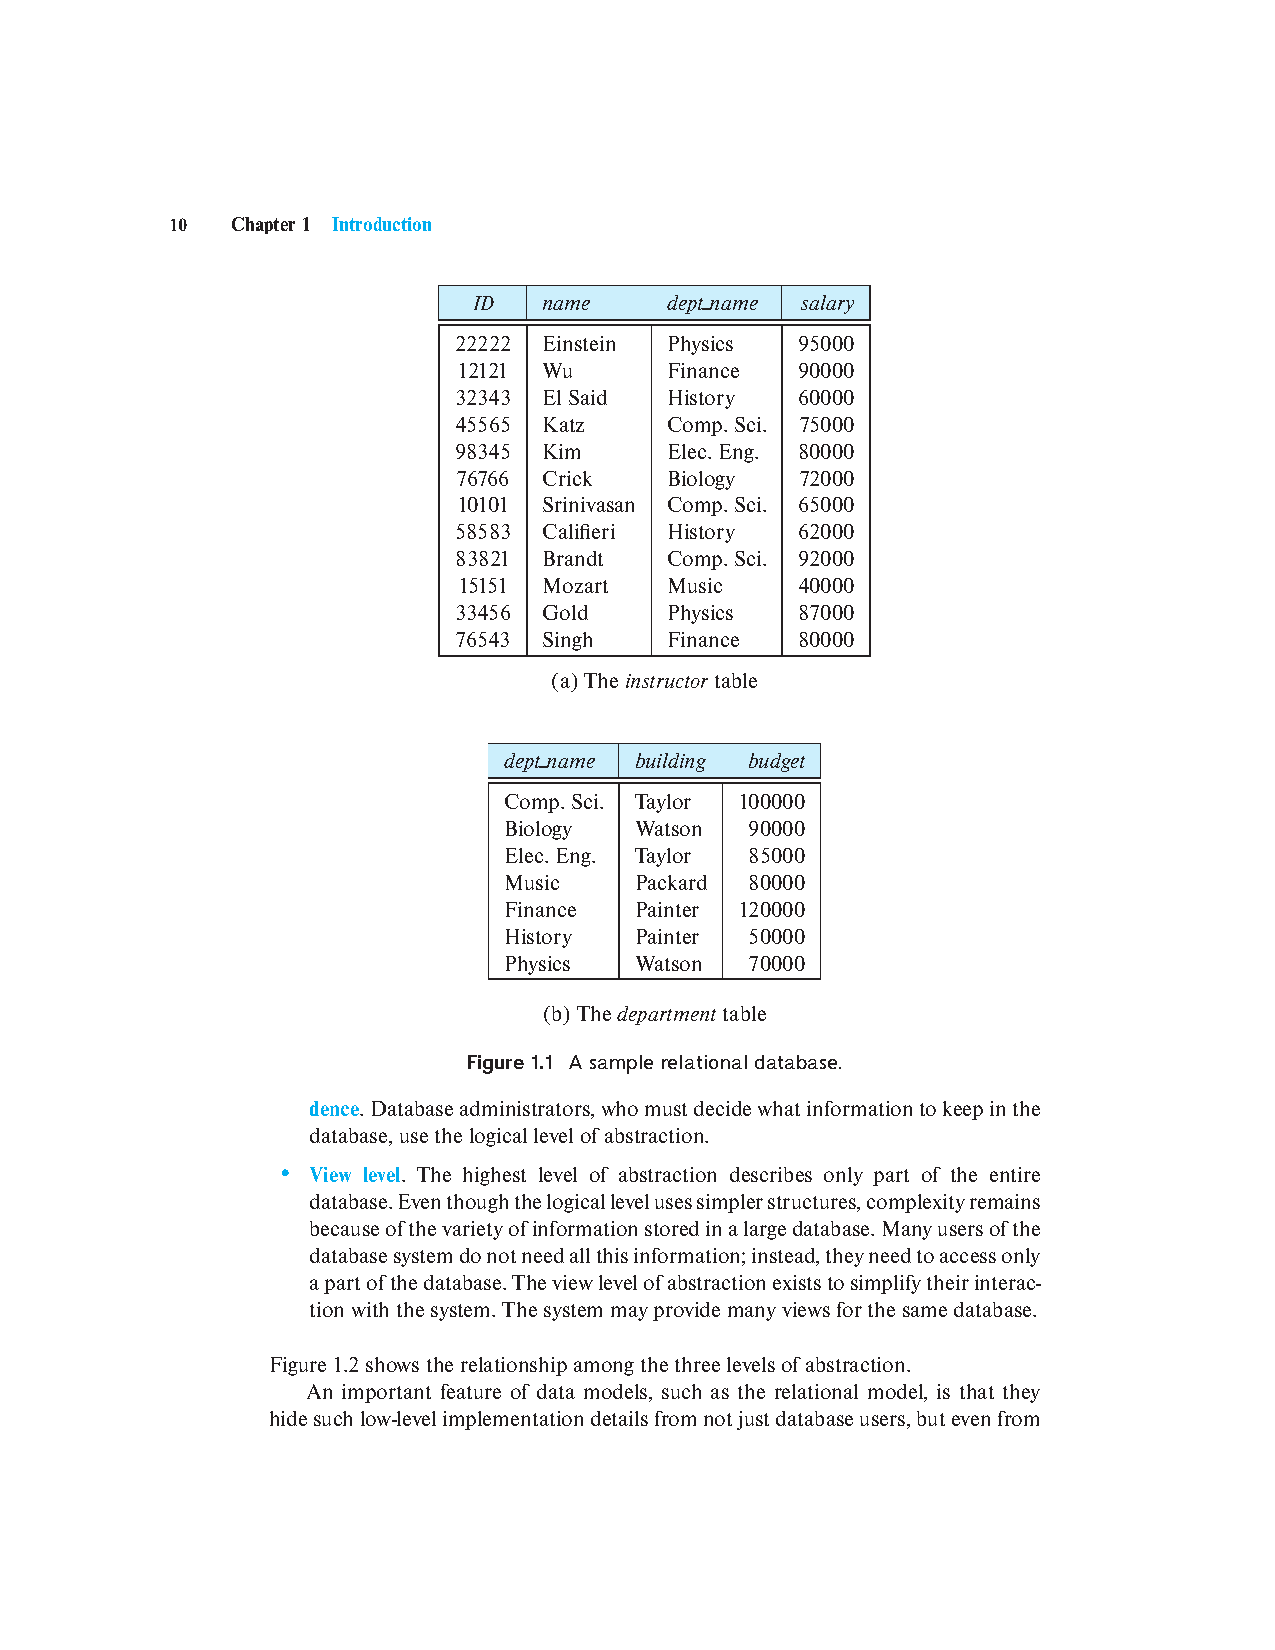
\includegraphics[width=0.45\textwidth, trim={7.25cm 5cm 6.75cm 4cm}, clip]{figures/db}
\end{frame}

\begin{frame}[fragile]{Levels of Abstraction}
    \begin{itemize}
        \item \textbf{Physical level:} describes how a record (e.g., instructor) is stored.
        \item \textbf{Logical level:} describes data stored in database, and the relationships among the data.
        \begin{Verbatim}[commandchars=\\\{\}]
        \userinput{type} instructor = \userinput{record} 
            ID: string;
            name: string;
            dept_name: string;
            salary: integer;
        \userinput{end};
        \end{Verbatim}
        \item \textbf{View level:} application programs hide details of data types.  Views can also hide information (such as an employee’s salary) for security purposes. 
    \end{itemize}
\end{frame}

\begin{frame}{Levels of Abstraction}
    The three levels of data abstraction.
    \centering 
    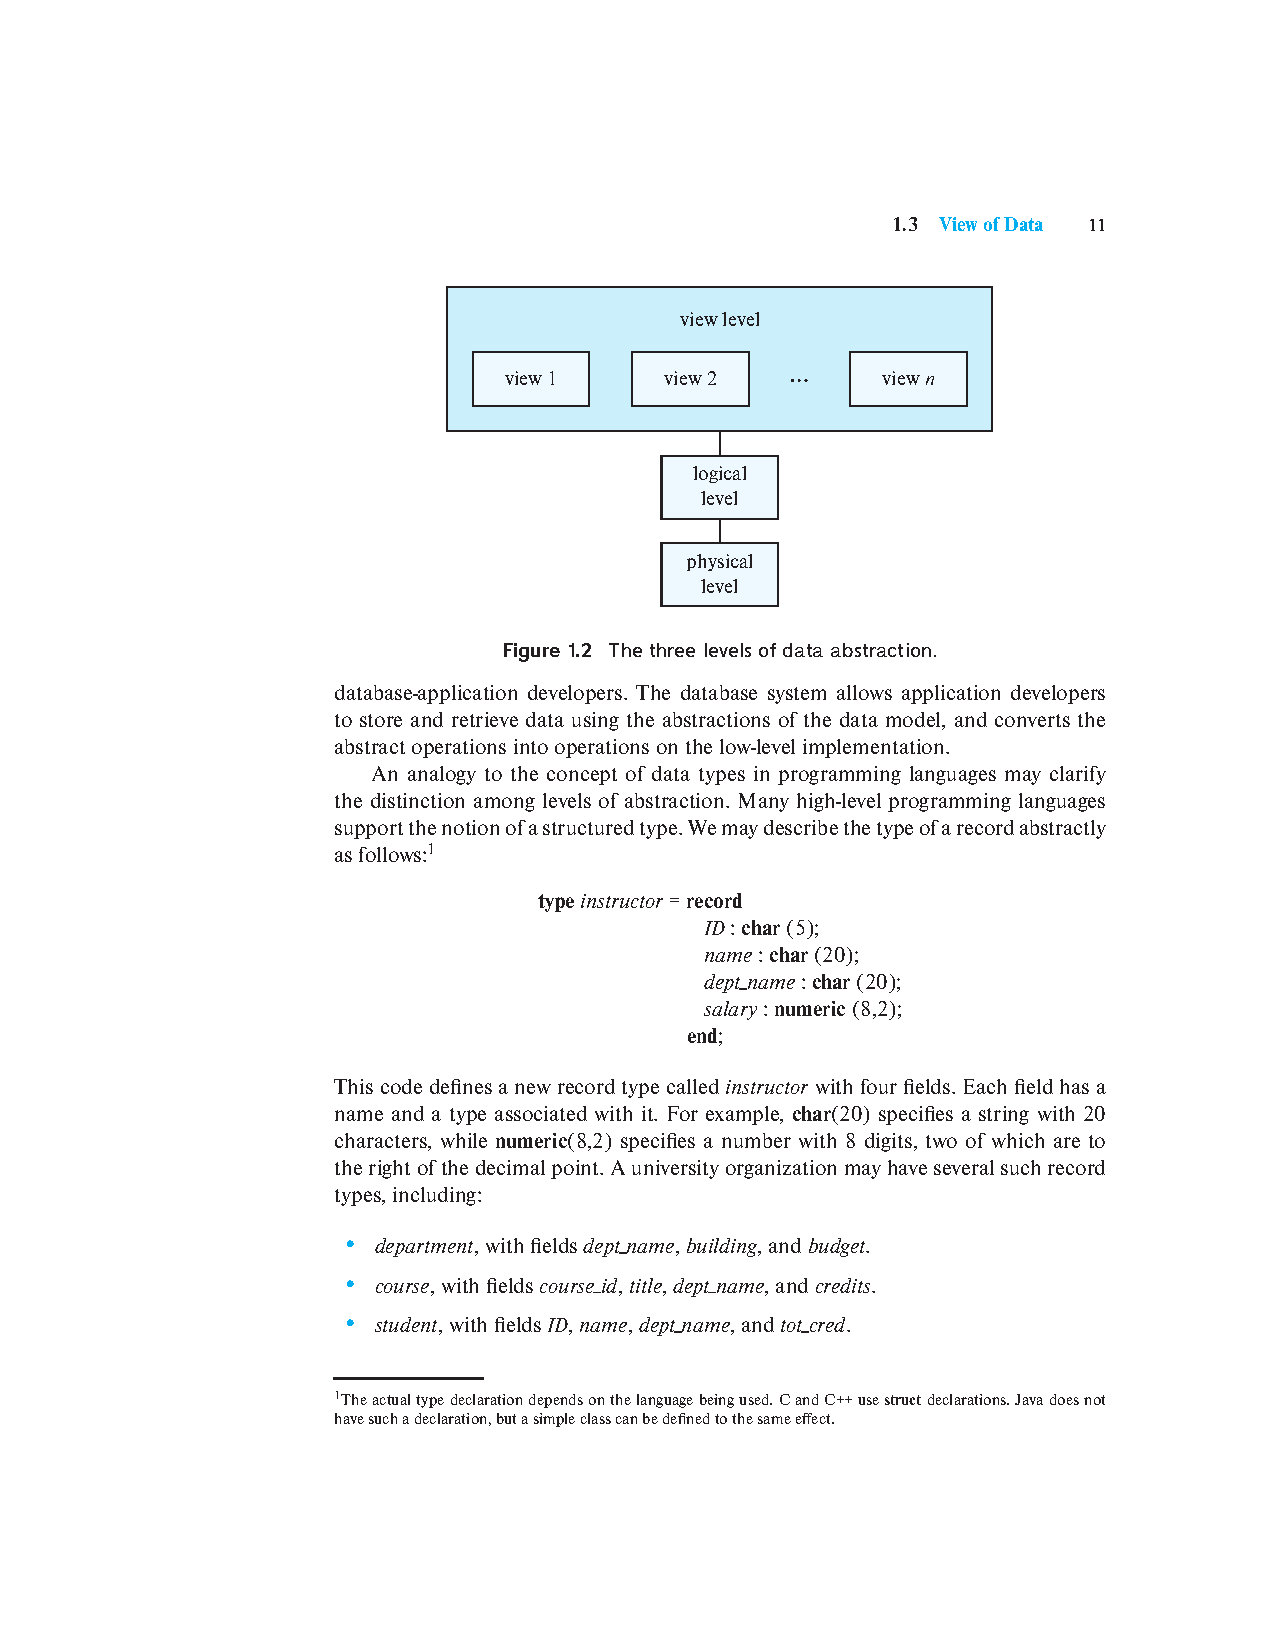
\includegraphics[width=0.9\textwidth, trim={7.25cm 17.5cm 4.75cm 4cm}, clip]{figures/arch}
\end{frame}

\begin{frame}{Instances and Schemas}
    \begin{itemize}
        \item Similar to types and variables in programming languages.
        \item \textbf{Logical Schema} --- the overall logical structure of the database:
        \begin{itemize}
            \item Example: The database consists of information about a set of customers and accounts in a bank and the relationship between them.
            \item Analogous to type information of a variable in a program.
        \end{itemize}
        \item \textbf{Physical Schema} --- the overall physical structure of the database.
        \item \textbf{Instance} --- the actual content of the database at a particular point in time.
        \begin{itemize}
            \item Analogous to the value of a variable.
        \end{itemize}
    \end{itemize}
\end{frame}

\begin{frame}{Physical Data Independence}
    \begin{itemize}
        \item \textbf{Physical Data Independence} --- the ability to modify the physical schema without changing the logical schema.
        \begin{itemize}
            \item Applications depend on the logical schema
            \item In general, the interfaces between the various levels and components should be well defined so that changes in some parts do not seriously influence others.
        \end{itemize}
    \end{itemize}
\end{frame}

\section{Database Languages}

\begin{frame}[fragile]{Data Definition Language (DDL)}
    \begin{itemize}
        \item Specification notation for defining the database schema.  Example:
        \begin{minted}[frame=lines, framesep=2mm, baselinestretch=1.2, bgcolor=LightGray, fontsize=\footnotesize, linenos]{sql}
    CREATE TABLE instructor(
        id varchar(5),
        name varchar(20),
        dept_name varchar(20),
        salary numeric(8,2)
    );
        \end{minted}
    \end{itemize}
\end{frame}

\begin{frame}{Data Definition Language (DDL)}
    \begin{itemize}
        \item DDL compiler generates a set of table templates stored in a \textbf{data dictionary}.
        \item Data dictionary contains metadata (i.e., data about data).
        \begin{itemize}
            \item Database schema.
            \item Integrity constraints: Primary key (ID uniquely identifies instructors).
            \item Authorization: Who can access what.
        \end{itemize}
    \end{itemize}
\end{frame}

\begin{frame}{Data Manipulation Language (DML)}
    \begin{itemize}
        \item Language for accessing and updating the data organized by the appropriate data model.
        \begin{itemize}
            \item DML also known as query language
        \end{itemize}
        \item There are basically two types of data-manipulation language:
        \begin{itemize}
            \item \textbf{Procedural DML} --- require a user to specify what data are needed and how to get those data.
            \item \textbf{Declarative DML} --- require a user to specify what data are needed without specifying how to get those data. 
        \end{itemize}
        \item Declarative DMLs are usually easier to learn and use than are procedural DMLs.  
        \item Declarative DMLs are also referred to as non-procedural DMLs.
        \item The portion of a DML that involves information retrieval is called a query language.  
    \end{itemize}
\end{frame}

\begin{frame}[fragile]{Standard Query Language (SQL)}
    \begin{itemize}
        \item SQL  query language is nonprocedural. A query takes as input several tables (possibly only one) and always returns a single table.
        \item Example to find all instructors in Comp. Sci. dept
        \begin{minted}
        [tabsize=4, obeytabs, frame=lines, framesep=2mm, baselinestretch=1.2, bgcolor=LightGray, fontsize=\footnotesize, linenos]
        {sql}
	SELECT
		name
	FROM 
		instructor
	WHERE
		dept_name = 'Comp. Sci.';
        \end{minted}
    \end{itemize}
\end{frame}

\begin{frame}[fragile]{Standard Query Language (SQL)}
    \begin{minted}
    [tabsize=4, obeytabs, frame=lines, framesep=2mm, baselinestretch=1.2, bgcolor=LightGray, fontsize=\footnotesize, linenos]
    {sql}
    SELECT
        instructor.ID, department.dept_name
    FROM 
        instructor, department
    WHERE
        instructor.dept_name = department.dept_name AND
        deptartment.budget >  95000;
    \end{minted}
\end{frame}

\begin{frame}{Standard Query Language (SQL)}
    \begin{itemize}
        \item SQL is \textbf{NOT} a Turing machine equivalent language.
        \item To be able to compute complex functions SQL is usually embedded in some higher-level language.
        \item Application programs generally access databases through one of:
        \begin{itemize}
            \item Language extensions to allow embedded SQL.
            \item Application program interface (e.g., ODBC/JDBC) which allow SQL queries to be sent to a database.
        \end{itemize}
    \end{itemize}
\end{frame}

\begin{frame}{Database Access from Application Program}
    \begin{itemize}
        \item Non-procedural query languages such as SQL are not as powerful as a universal Turing machine.    
        \item SQL does not support actions such as input from users, output to displays, or communication over the network.  
        \item Such computations and actions must be written in a host language, such as C/C++, Java or Python, with embedded SQL queries that access the data in the database.
        \item Application programs --- are programs that are used to interact with the database in this fashion.  
    \end{itemize}
\end{frame}

\section{Database Design}

\begin{frame}{Database Design}
The process of designing the general structure of the database:
    \begin{itemize}
        \item Logical Design --- Deciding on the database schema. Database design requires that we find a “good” collection of relation schemas.
        \begin{itemize}
            \item Business decision -- What attributes should we record in the database?
            \item Computer Science decision --  What relation schemas should we have and how should the attributes be distributed among the various relation schemas?
        \end{itemize}
        \item Physical Design --- Deciding on the physical layout of the database                
    \end{itemize}
\end{frame}

\begin{frame}{Database Engine}
    \begin{itemize}
        \item A database system is partitioned into modules that deal with each of the responsibilities of the overall system.  
        \item The functional components of a database system can be divided into:
        \begin{itemize}
            \item The storage manager.
            \item The  query processor component.
            \item The transaction management component.
        \end{itemize}
    \end{itemize}
\end{frame}

\begin{frame}{Storage Manager}
    \begin{itemize}
        \item A program module that provides the interface between the low-level data stored in the database and the application programs and queries submitted to the system.
        \item The storage manager is responsible to the following tasks: 
        \begin{itemize}
            \item Interaction with the OS file manager.
            \item Efficient storing, retrieving and updating of data.
        \end{itemize}
        \item The storage manager components include:
        \begin{itemize}
            \item Authorization and integrity manager.
            \item Transaction manager.
            \item File manager.
            \item Buffer manager.
        \end{itemize}
    \end{itemize}
\end{frame}

\begin{frame}{Storage Manager (Cont.)}
    \begin{itemize}
        \item The storage manager implements several data structures as part of the physical system implementation:
        \begin{itemize}
            \item Data files -- store the database itself.
            \item Data dictionary --  stores metadata about the structure of the database, in particular the schema of the database.
            \item Indices --  can provide fast access to data items.  A database index provides pointers to those data items that hold a particular value.
        \end{itemize}
    \end{itemize}
\end{frame}

\begin{frame}{Query Processor}
    \begin{itemize}
        \item The query processor components include:
        \begin{itemize}
            \item DDL  interpreter --  interprets DDL statements and records the definitions in the data dictionary.
            \item DML compiler -- translates DML statements in a query language into an \textit{evaluation plan} consisting of low-level instructions that the query evaluation engine understands.
            \begin{itemize}
                \item The DML compiler performs query optimization; that is, it picks the lowest cost evaluation plan from among the various alternatives.
            \end{itemize}
            \item Query evaluation engine -- executes low-level instructions generated by the DML compiler.
        \end{itemize}
    \end{itemize}
\end{frame}

\begin{frame}{Query Processing}
    \begin{itemize}
        \item Parsing and translation.
        \item Optimization.
        \item Evaluation.
    \end{itemize}
    \centering 
    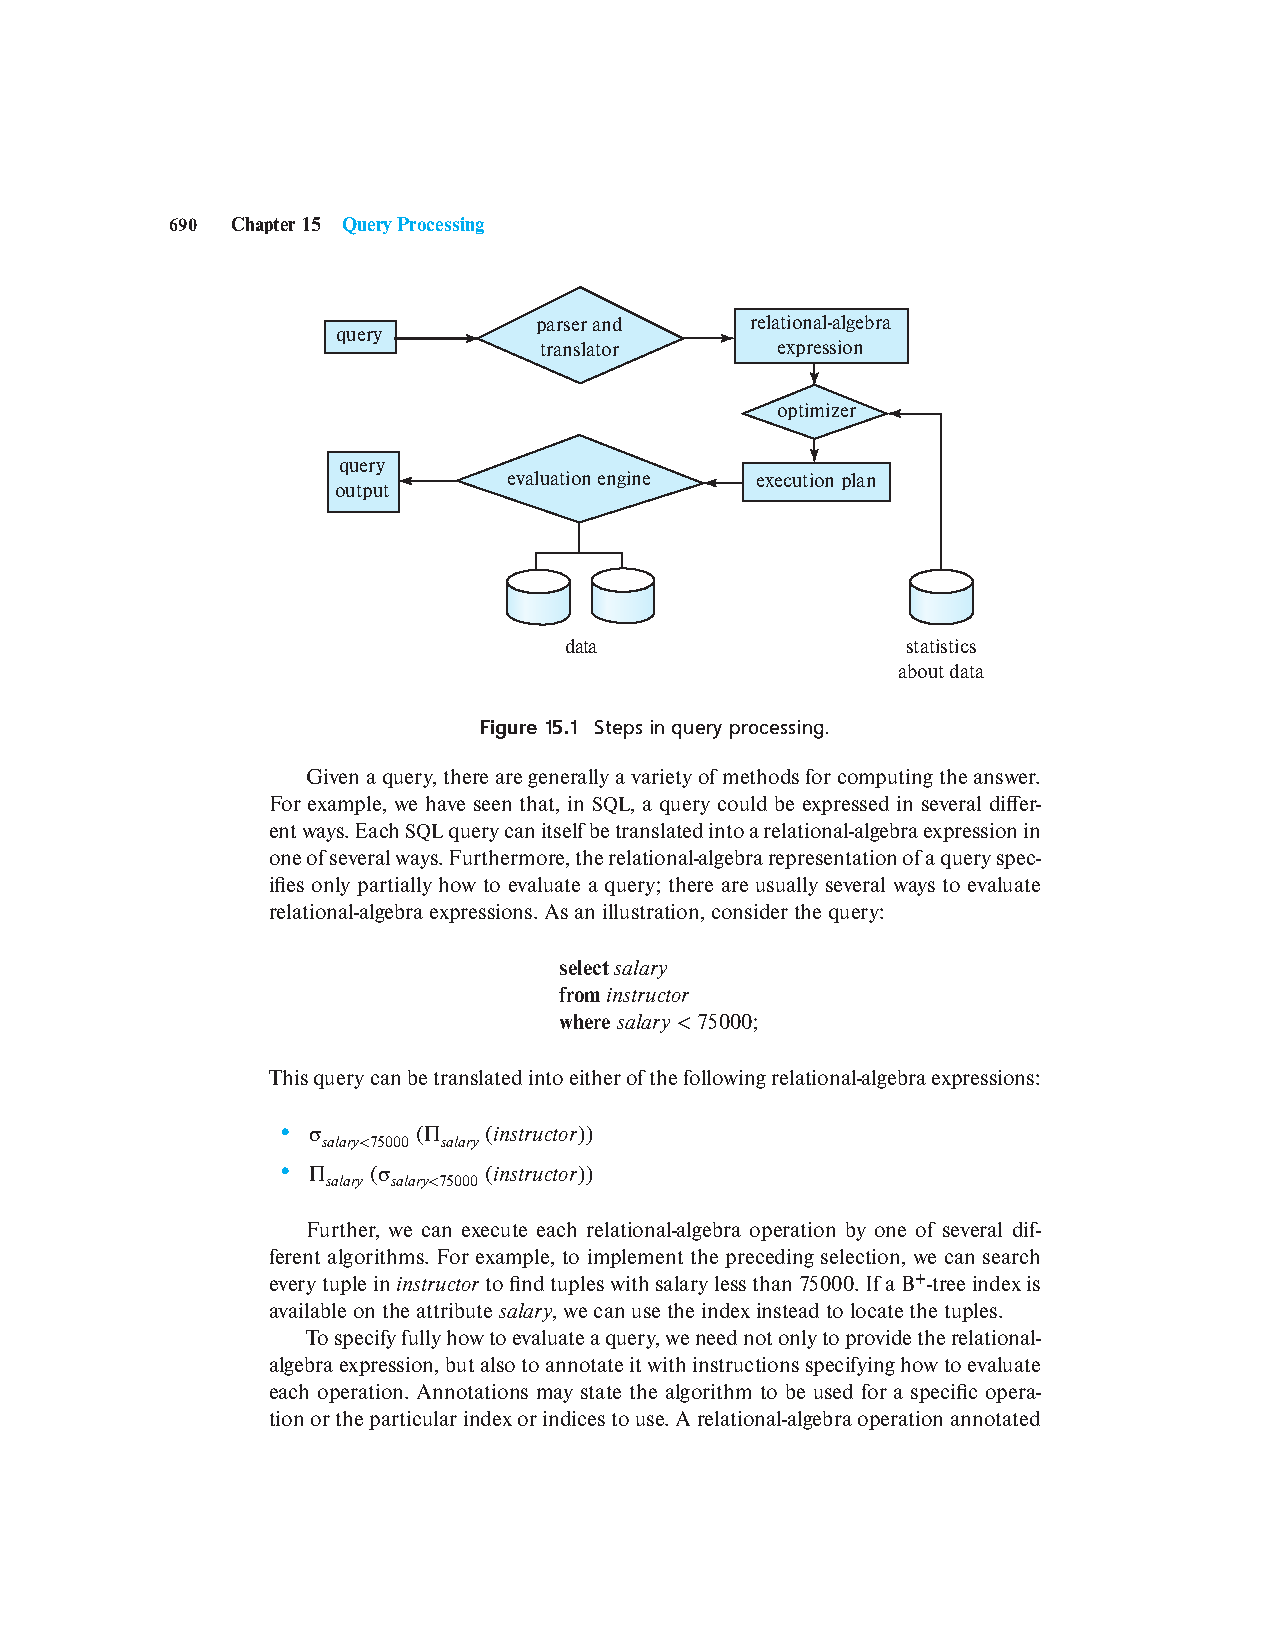
\includegraphics[width=\textwidth, trim={5.25cm 16.25cm 4.9cm 4.5cm}, clip]{figures/qp}
\end{frame}

\begin{frame}{Transaction Management	}
    \begin{itemize}
        \item A \textbf{transaction} is a collection of operations that performs a single logical function in a database application
        \item \textbf{Transaction-management component} ensures that the database remains in a consistent (correct) state despite system failures (e.g., power failures and operating system crashes) and transaction failures.
        \item \textbf{Concurrency-control manager} controls the interaction among the concurrent transactions, to ensure the consistency of the database.
    \end{itemize}
\end{frame}

\section{Database and Application Architecture}

\begin{frame}{Database Architecture}
    \begin{itemize}
        \item Centralized databases:
        \begin{itemize}
            \item One to a few cores, shared memory.
        \end{itemize}
        \item Client-server:
        \begin{itemize}
            \item One server machine executes work on behalf of multiple client machines.
        \end{itemize}
        \item Parallel databases:
        \begin{itemize}
            \item Many core shared memory.
            \item Shared disk.
            \item Shared nothing.
        \end{itemize}
        \item Distributed databases:
        \begin{itemize}
            \item Geographical distribution.
            \item Schema/data heterogeneity.
        \end{itemize}
    \end{itemize}
\end{frame}

\begin{frame}{Database Architecture (Centralized/Shared-Memory)}
    \centering 
    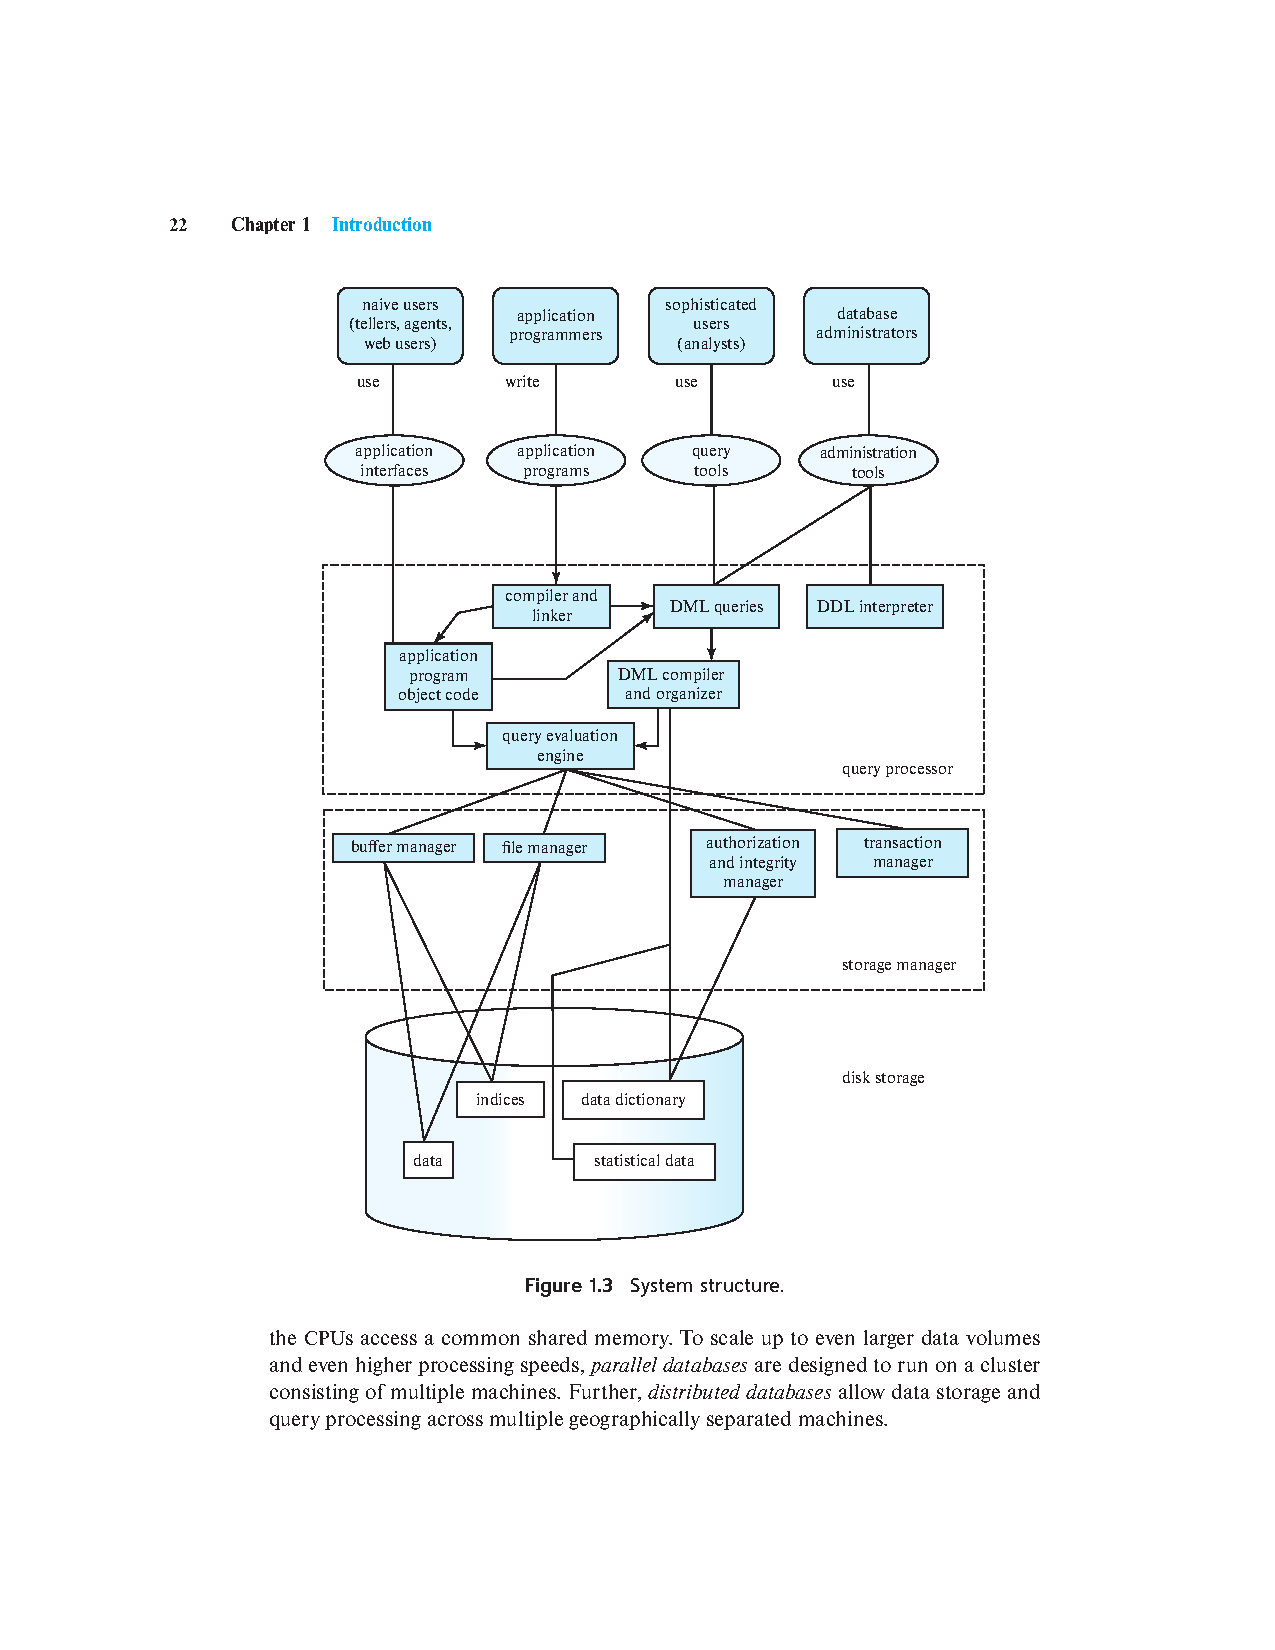
\includegraphics[width=0.625\textheight, trim={5.25cm 6.75cm 4.9cm 4.8cm}, clip]{figures/arch2}
\end{frame}

\begin{frame}{Database Architecture (Centralized/Shared-Memory)}
    \centering 
    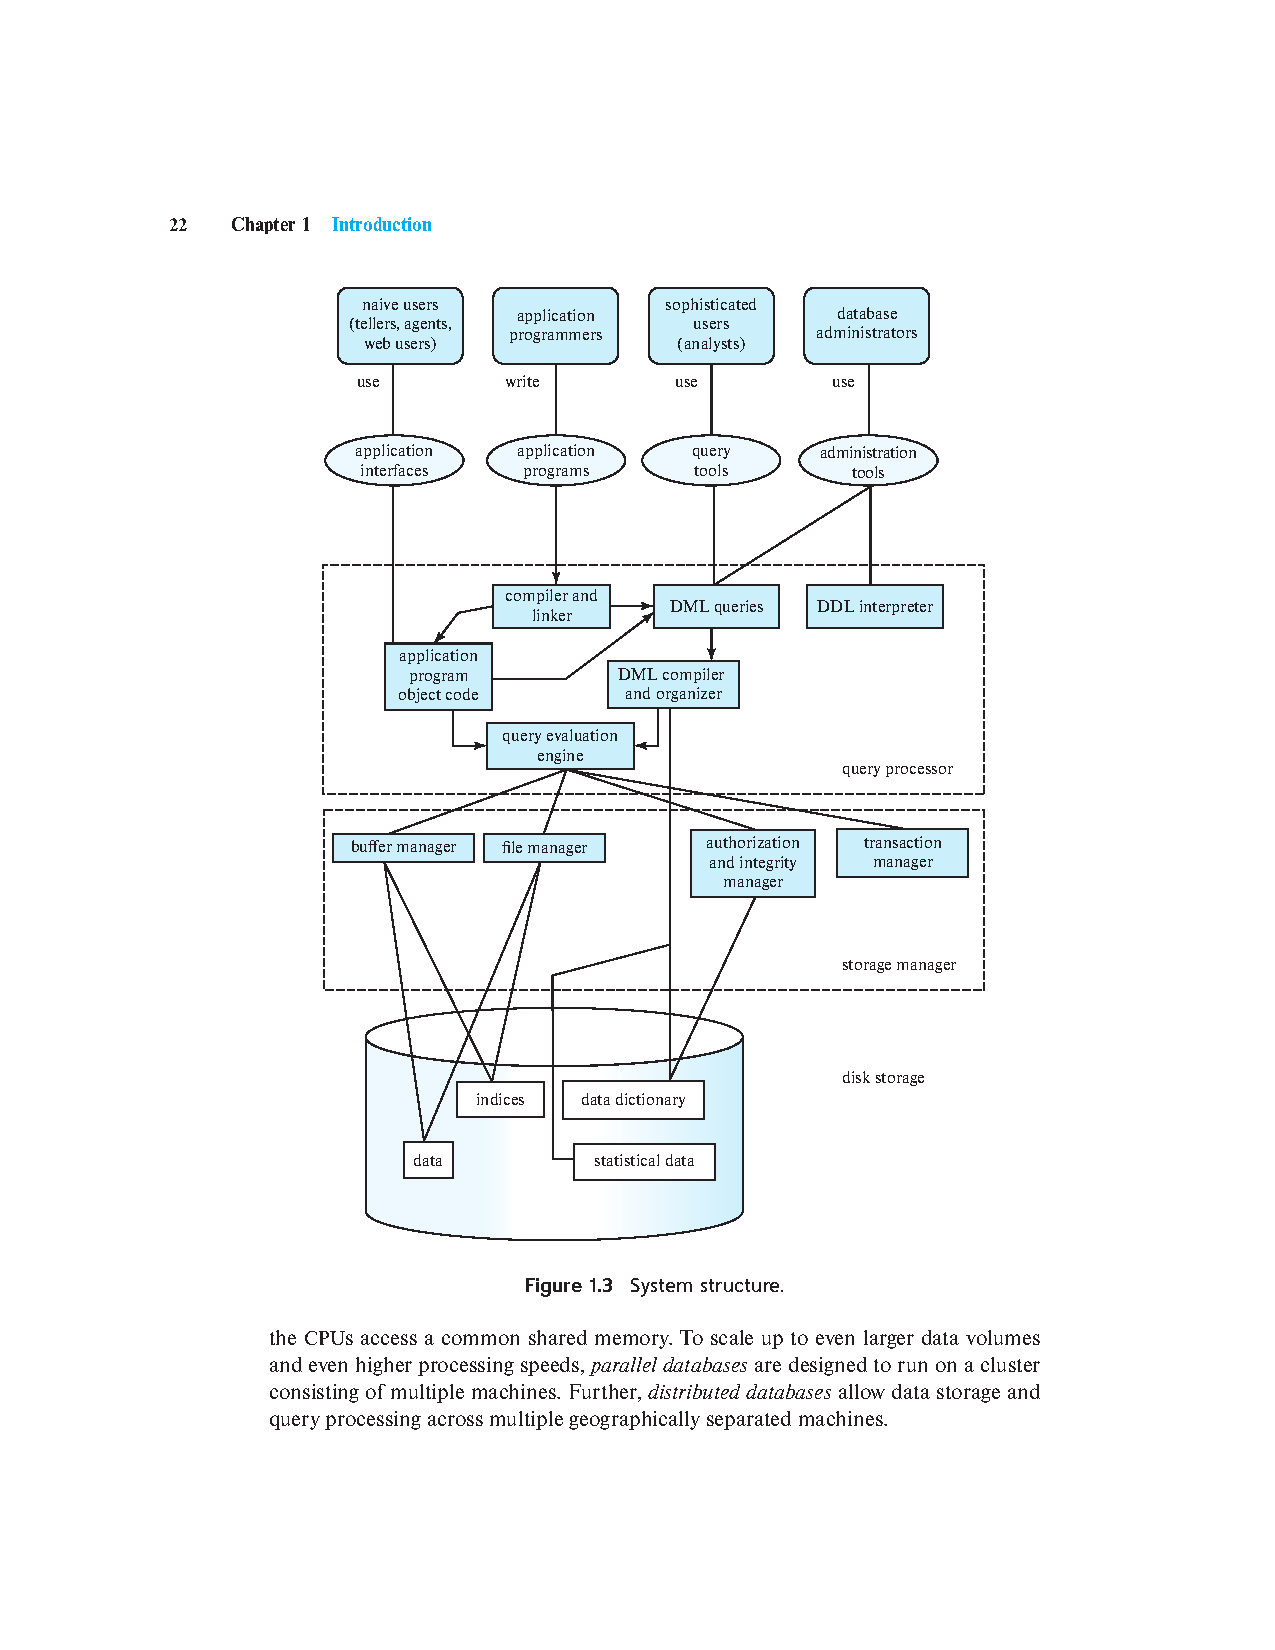
\includegraphics[width=0.85\textheight, trim={5.25cm 6.75cm 4.9cm 9.55cm}, clip]{figures/arch2}
\end{frame}

\begin{frame}{Database Applications}
Database applications are usually partitioned into two or three parts:
    \begin{itemize}
        \item Two-tier architecture --  the application resides at the client machine, where it invokes database system functionality at the server machine.
        \item Three-tier architecture -- the client machine acts as a front end and does not contain any direct database calls.
        \begin{itemize}
            \item The client end communicates with an application server, usually through a forms interface.  
            \item The application server in turn communicates with a database system to access data.
        \end{itemize}
    \end{itemize}
\end{frame}

\begin{frame}{Two-tier and three-tier architectures}
    \centering 
    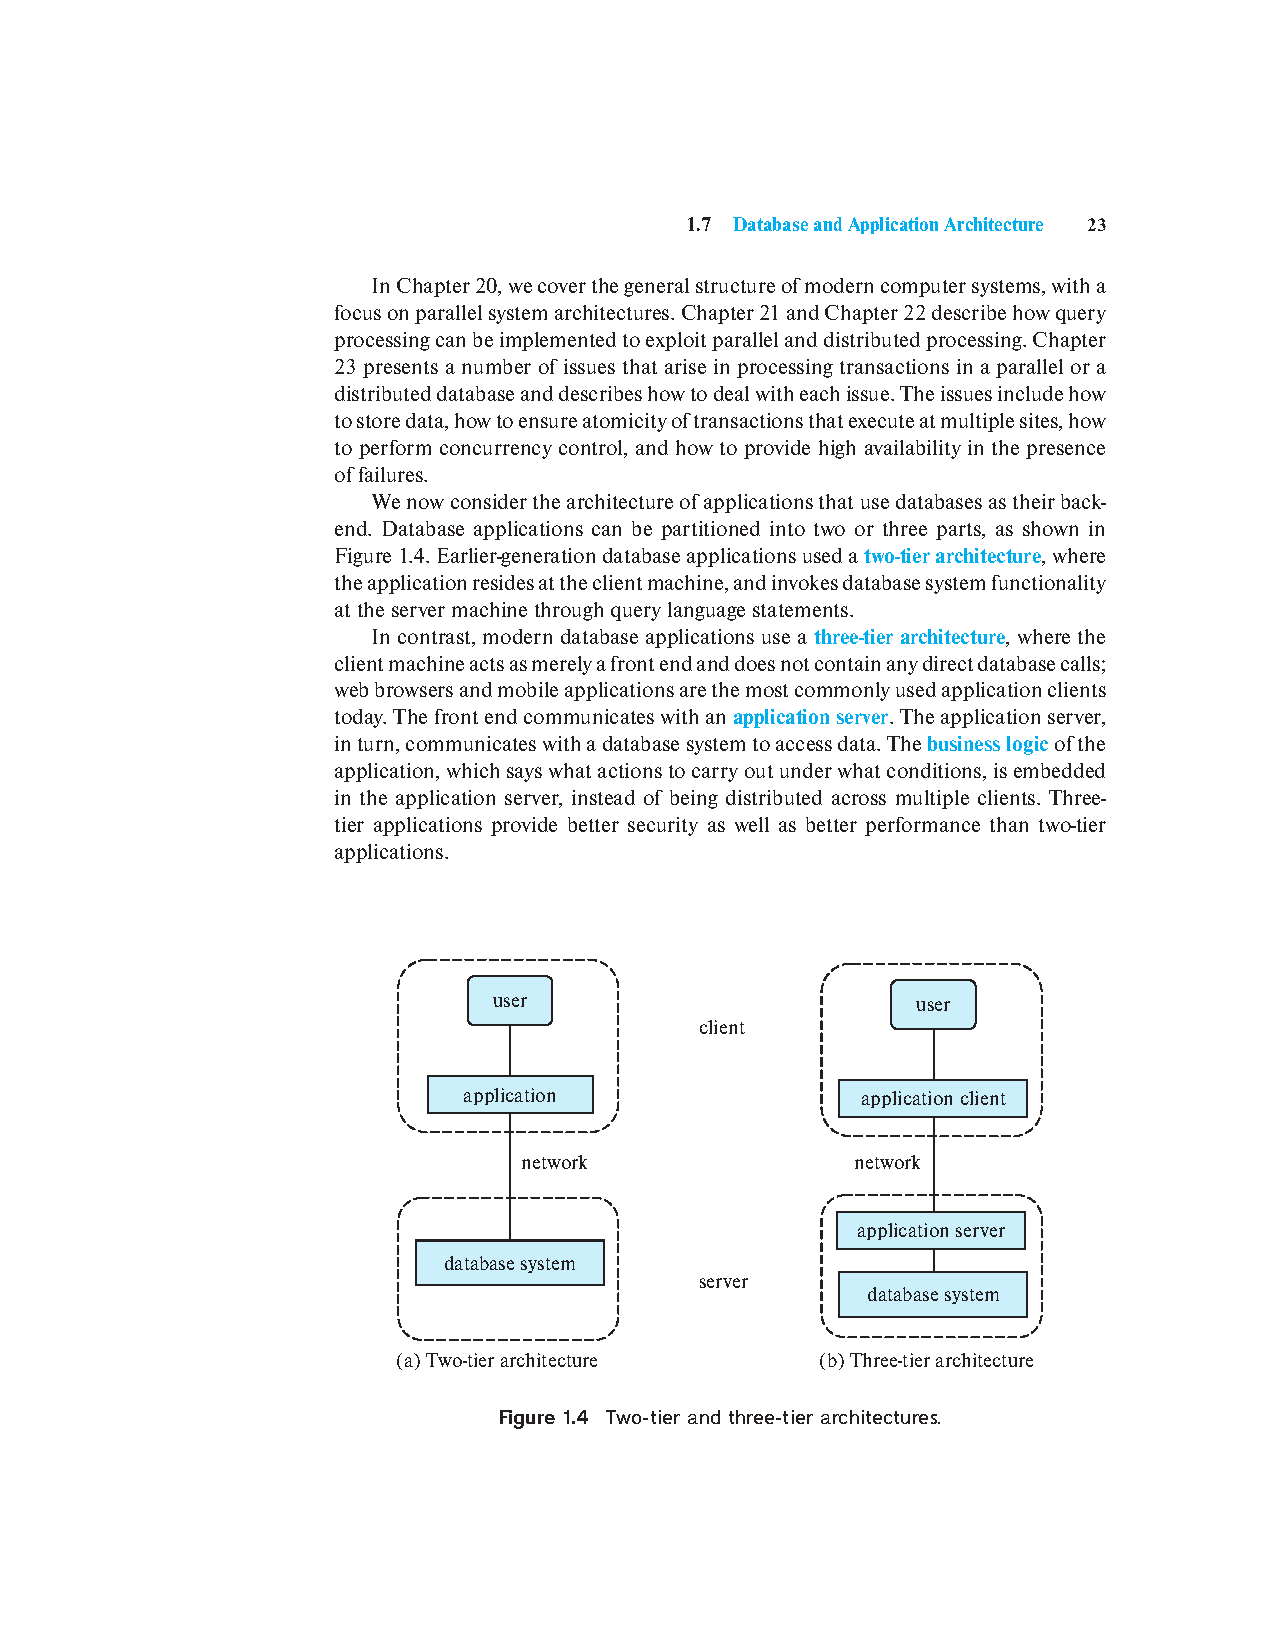
\includegraphics[width=\textheight, trim={6cm 4.25cm 3.8cm 16.25cm}, clip]{figures/tiers}
\end{frame}

\section{Database Users and Administrators}

\begin{frame}{Database Users and User Interfaces}
    \centering 
    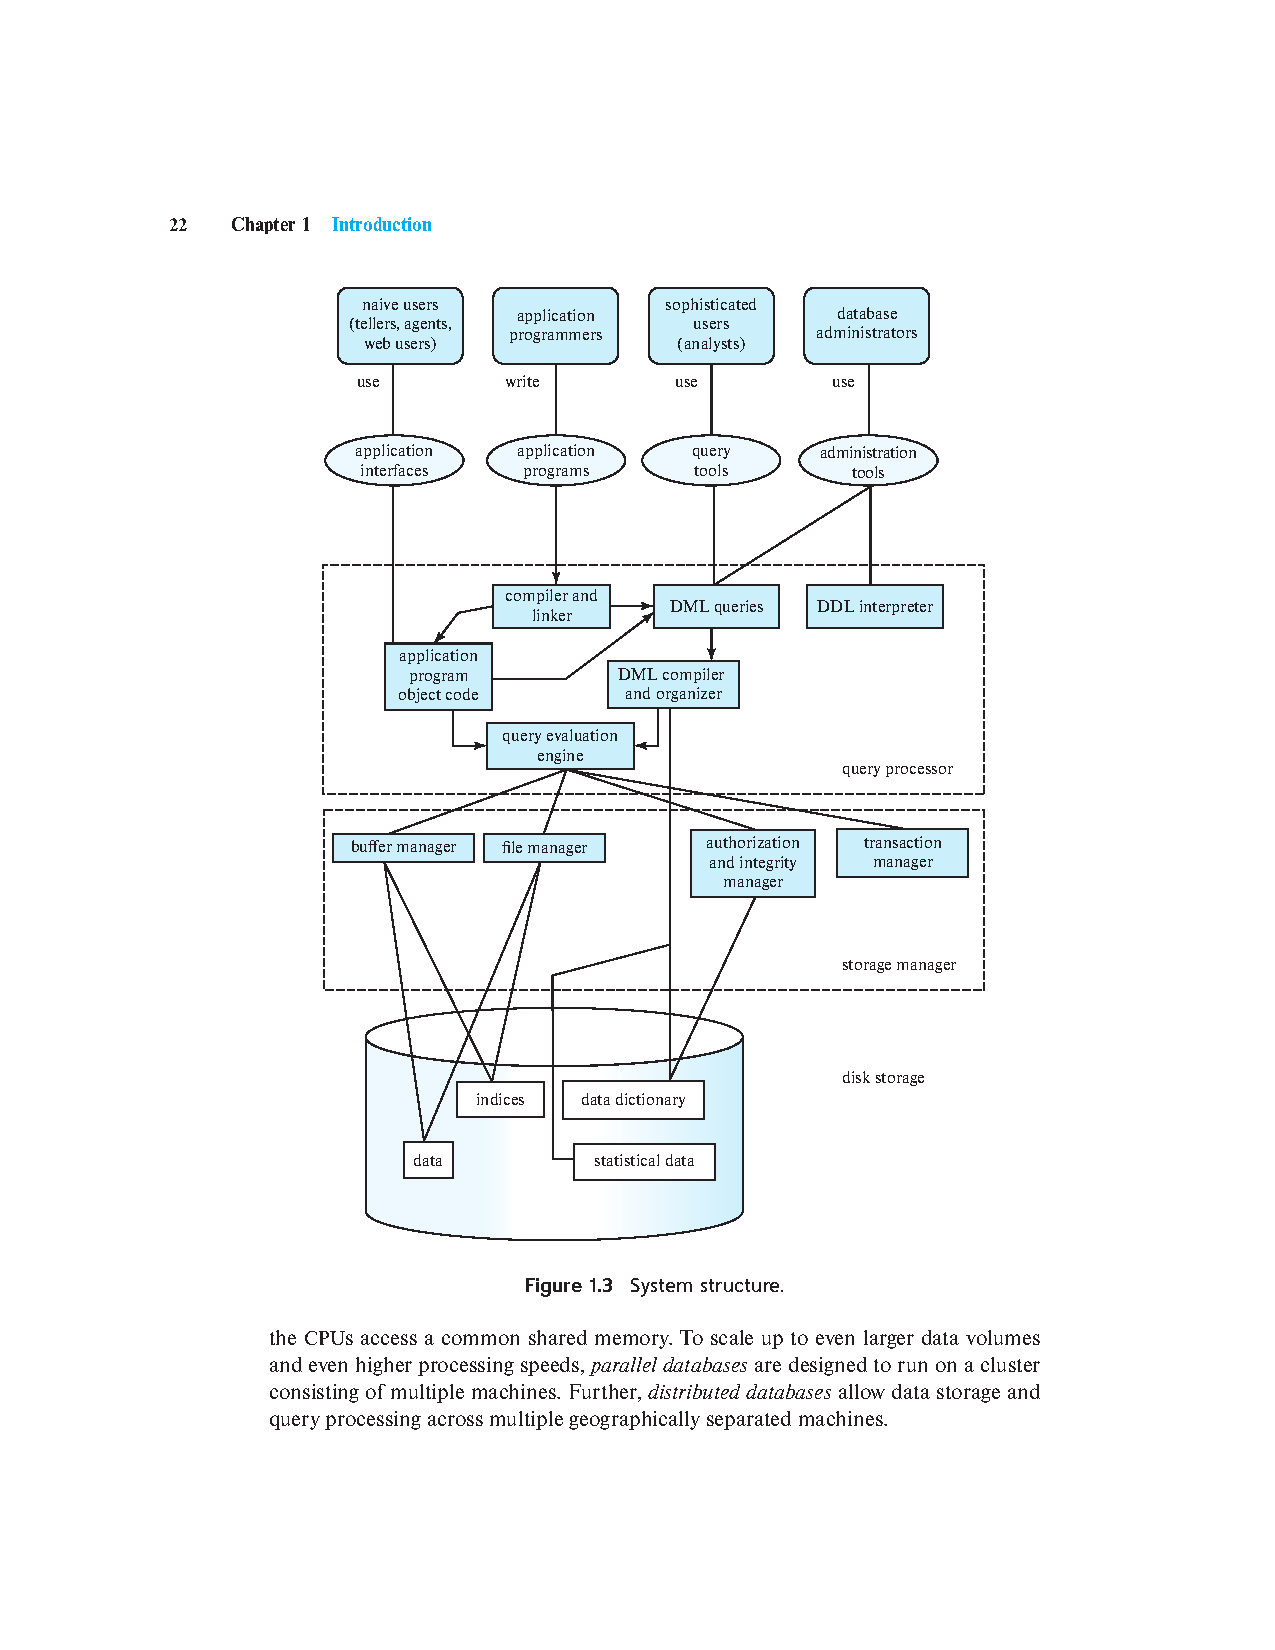
\includegraphics[width=0.625\textheight, trim={5.25cm 6.75cm 4.9cm 4.8cm}, clip]{figures/arch2}
\end{frame}

\begin{frame}{Database Users  and User Interfaces}
    \centering 
    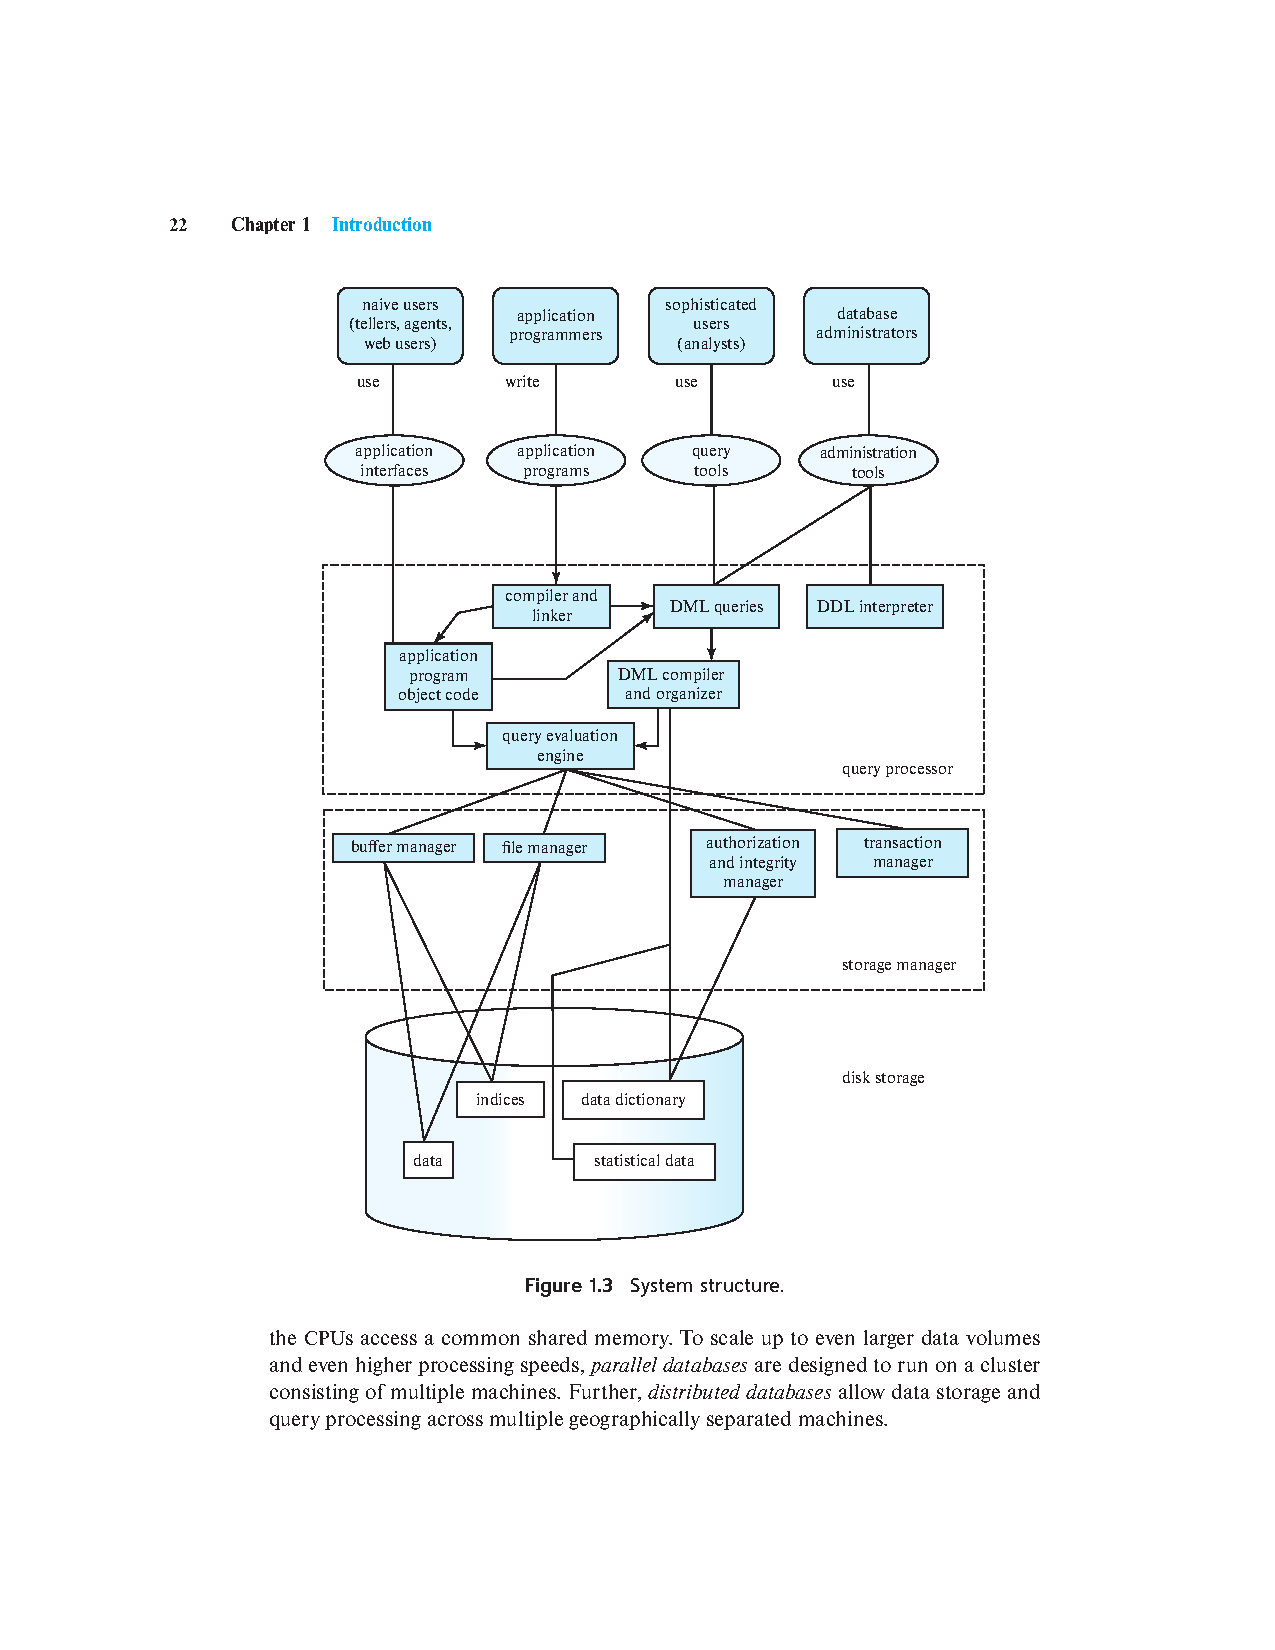
\includegraphics[width=0.85\textheight, trim={5.25cm 14.475cm 4.9cm 4.8cm}, clip]{figures/arch2}
\end{frame}

\begin{frame}{Database Administrator}
A person who has central control over the system is called a \textbf{Database Administrator (DBA)}.  Functions of a DBA include:
    \begin{itemize}
        \item Schema definition.
        \item Storage structure and access-method definition.
        \item Schema and physical-organization modification.
        \item Granting of authorization for data access.
        \item Routine maintenance.
        \item Periodically backing up the database.
        \item Ensuring that enough free disk space is available for normal operations, and upgrading disk space as required.
        \item Monitoring jobs running on the database.
    \end{itemize}
\end{frame}

\section{History of Database Systems}

\begin{frame}{History of Database Systems}
    \begin{itemize}
        \item 1950s and 60s: Magnetic tapes and punched cards...
        \item 1970s: Relational model introduced by Ted Codd...
        \item 1980s: Commercialization of relational databases...
        \item 1990s: Data warehouses and data mining...
        \item 2000s: Big data systems (NoSQL, MapReduce)...
    \end{itemize}
\end{frame}

\section*{Takeaways}

\begin{frame}{TDT5FTOTC}
    \centering
    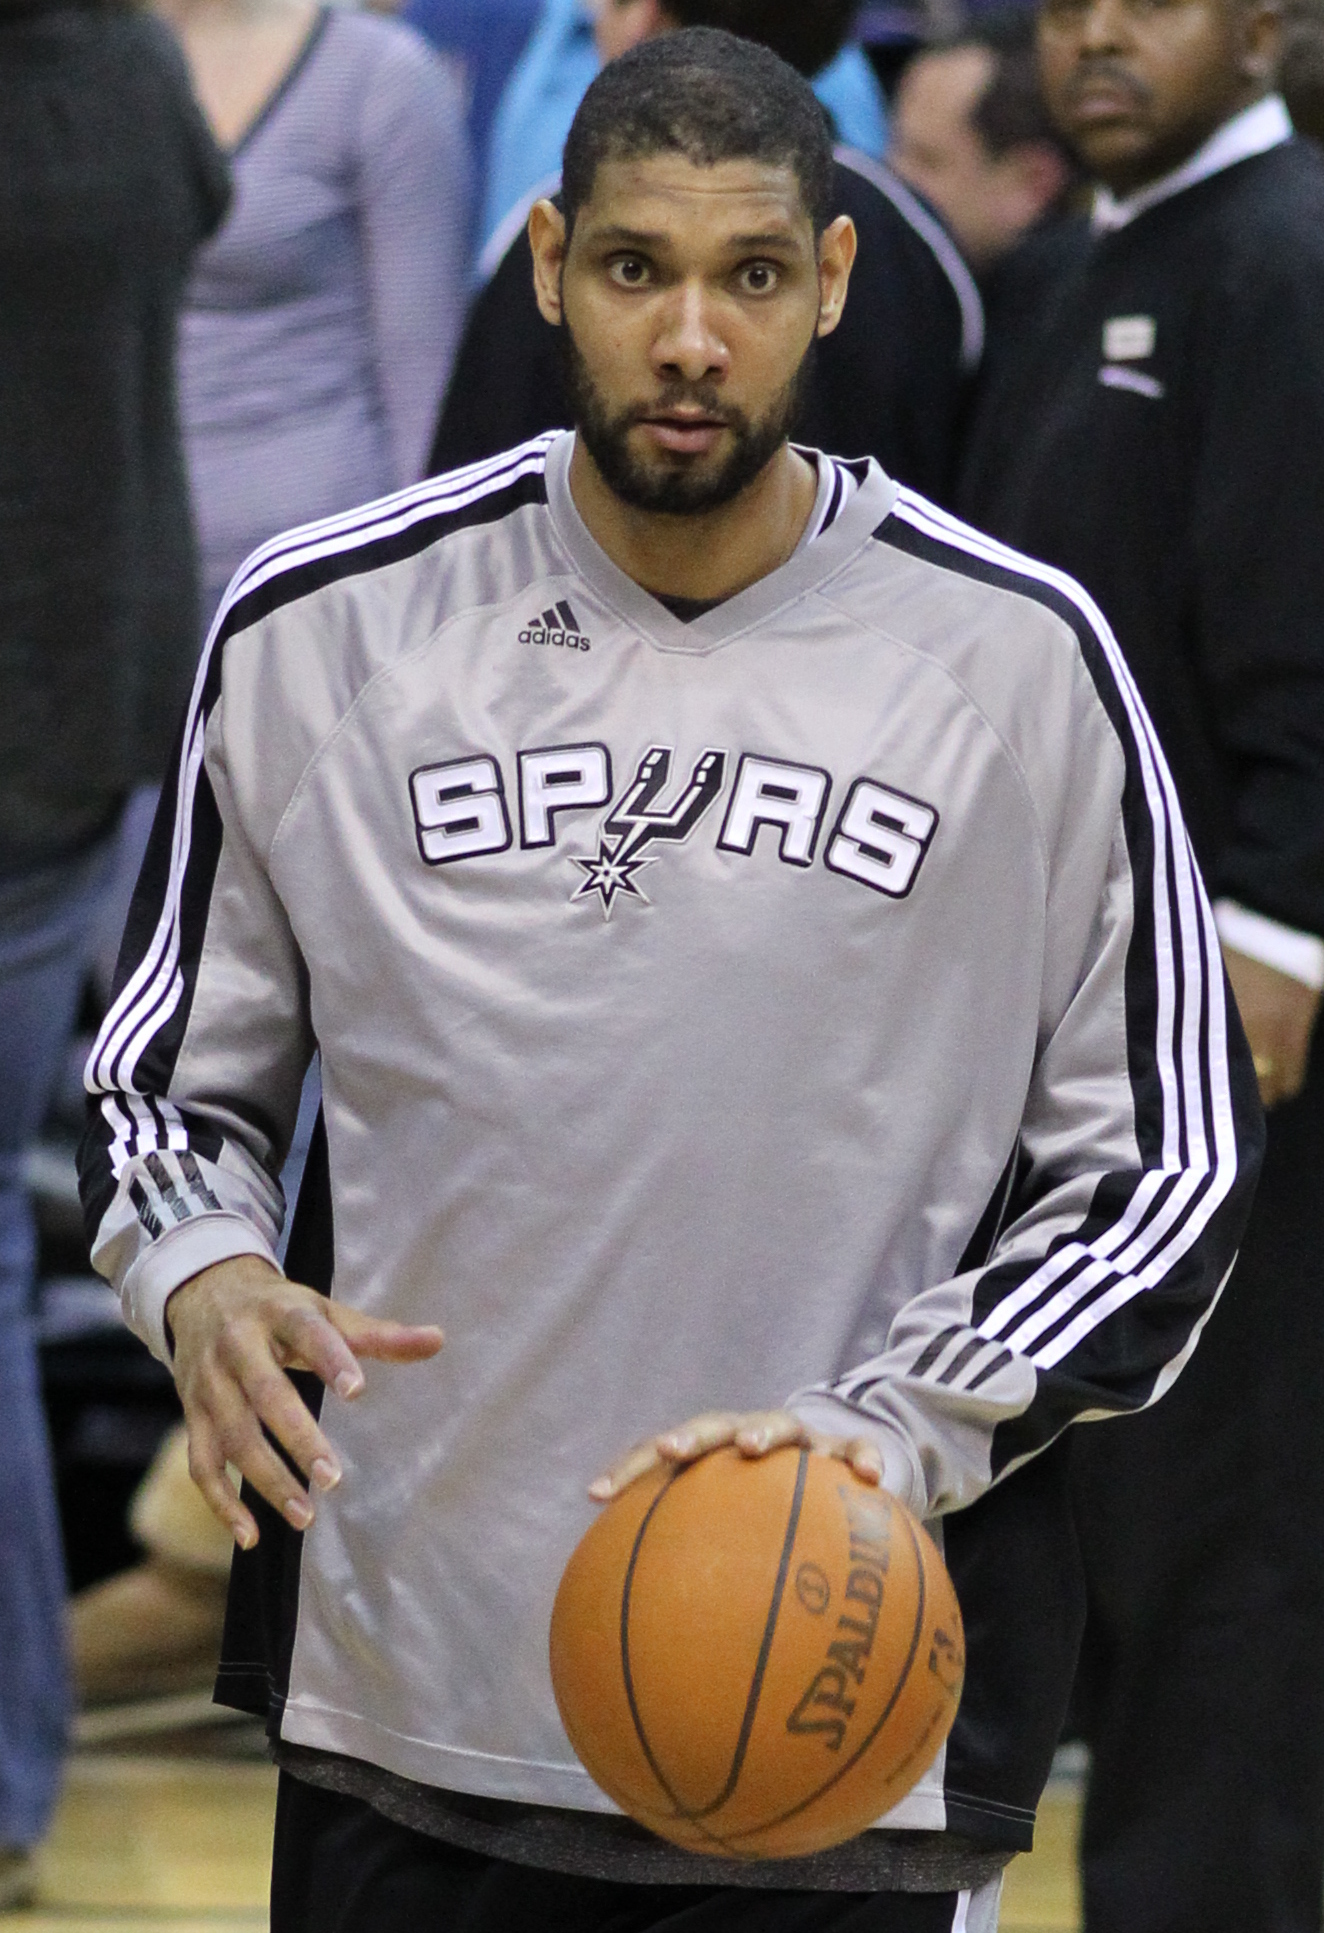
\includegraphics[width=0.45\textwidth]{figures/td.jpg}\\
    \href{https://en.wikipedia.org/wiki/Tim_Duncan}{Tim Duncan in Wikipedia.}
\end{frame}

% Tim Duncan's Top 5 Fundamental Takeaways of the Today's Class
\begin{frame}{TDT5FTOTTC}
    \centering
    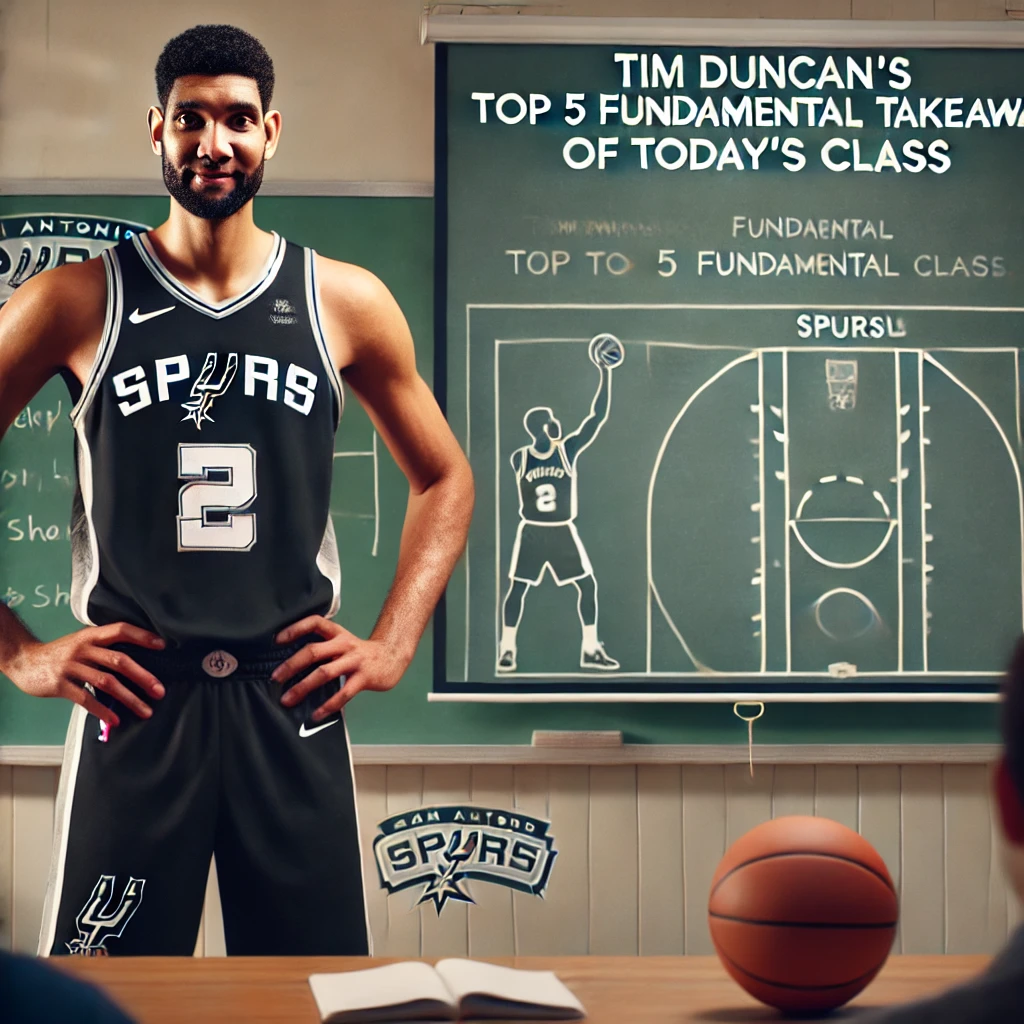
\includegraphics[width=0.75\textwidth]{figures/tim.png}
\end{frame}

\begin{frame}{Top 5 Fundamental Takeaways}
    \begin{enumerate} \pause
        \item[5] \textbf{Evolution of DBMS:} Database systems have advanced from simple file-processing systems to distributed and cloud-based solutions. \pause
        \item[4] \textbf{Purpose of DBMS:} A DBMS ensures efficient, secure, and reliable management of data while addressing redundancy and inconsistency. \pause
        \item[3] \textbf{Database Applications:} Databases are integral to transaction processing, data analytics, and modern big data environments. \pause
        \item[2] \textbf{Database Languages:} DBMS uses DDL for defining structures and DML for querying and modifying data effectively. \pause
        \item[1] \textbf{Data Abstraction:} It provides physical, logical, and view-level abstractions to simplify user interaction and system complexity. 
    \end{enumerate}
\end{frame}

\begin{frame}{}
    \centering
    \Huge End of Chapter 1.
\end{frame}

\begin{frame}{Database System Concepts}
    \centering
    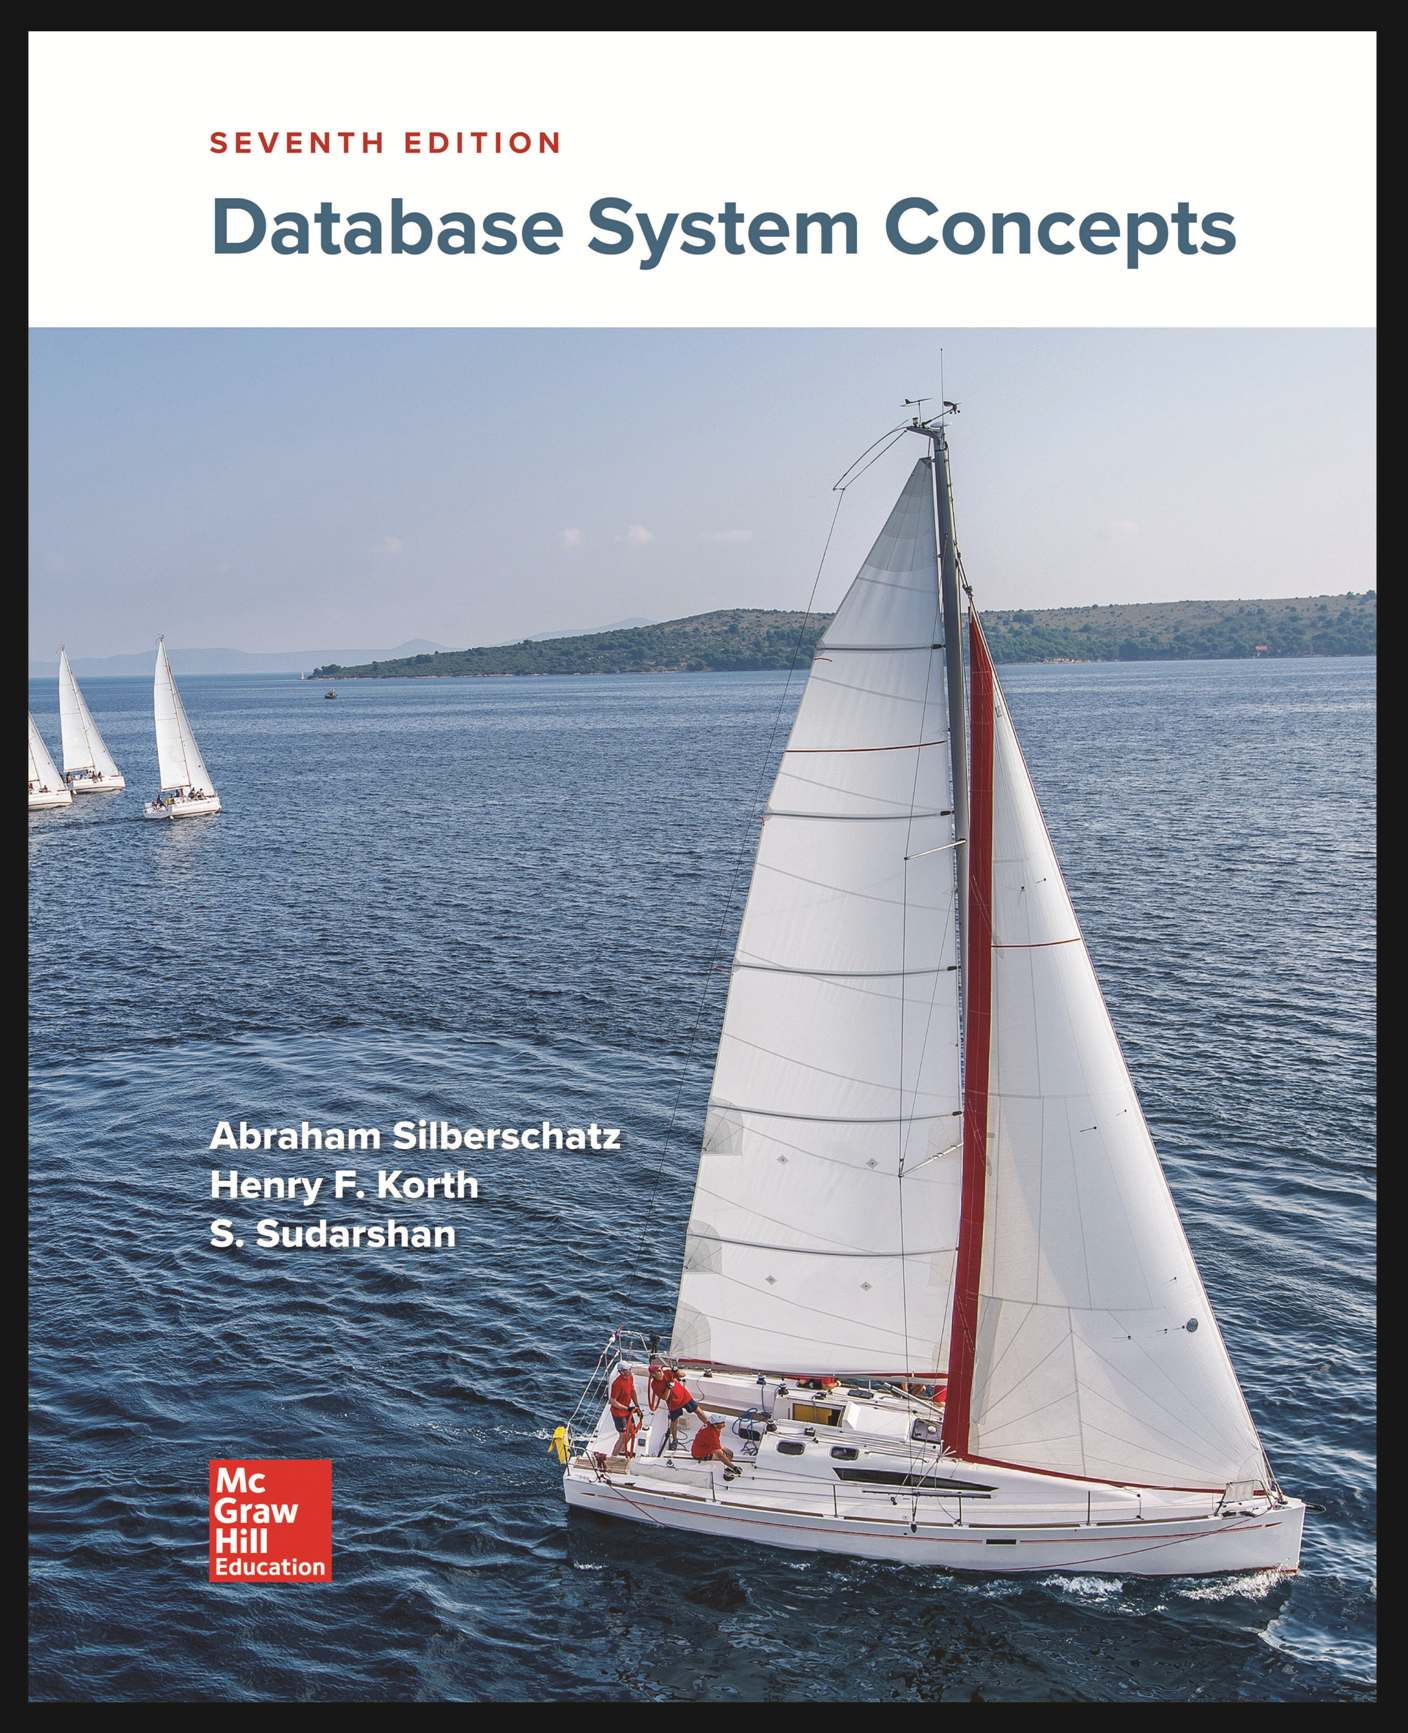
\includegraphics[width=0.5\textwidth]{figures/book_cover.jpg} \\
    \vspace{5mm}
    {
        \tiny
        Content has been extracted from \textit{Database System Concepts}, Seventh Edition, by Silberschatz, Korth and Sudarshan. Mc Graw Hill Education. 2019.\\
        Visit \url{https://db-book.com/}.\\
    }
\end{frame}

\end{document}
